% =========================================================================
% DepthStream 中文版（对应 main.tex 英文版 v2 叙事）
% 编译：xelatex main_zh.tex （两遍）
% =========================================================================
\documentclass[10pt,twocolumn]{article}
\usepackage[margin=0.75in,columnsep=0.25in]{geometry}
\usepackage{amsmath,amssymb}
\usepackage{graphicx}
\usepackage{booktabs}
\usepackage{multirow}
\usepackage{microtype}
\usepackage{xcolor}
\usepackage[colorlinks=true,linkcolor=blue,citecolor=blue,urlcolor=blue]{hyperref}
\usepackage{xeCJK}
\setCJKmainfont{Noto Serif CJK SC}
\setCJKsansfont{Noto Sans CJK SC}
\setCJKmonofont{Noto Sans CJK SC}
\renewcommand{\abstractname}{摘要}
\renewcommand{\figurename}{图}
\renewcommand{\tablename}{表}
\renewcommand{\refname}{参考文献}
\graphicspath{{figs/}}

\newcommand{\Dhat}{\hat{D}}
\newcommand{\Dprev}{D_{t-1}}
\newcommand{\Dphi}{D^{\phi}_{t}}

\title{\LARGE\bf DepthStream：视频深度时间一致性的免费午餐}
\author{匿名（中文预印本，对应英文稿 v2）\\ \small 代码与评测：\texttt{eval\_sintel\_v2.py / eval\_bonn.py / bench\_cpu.py}}
\date{}

\begin{document}
\sloppy
\maketitle

%--------------------------------------------------------------------------
\begin{abstract}
视频深度的时间一致性从来都是有偿的——要么牺牲精度，要么牺牲算力，要么付出训练代价：最强的传播式系统围绕基础模型学习一个修正模块，其代价是数天的 GPU 训练和旗舰级 GPU 运行时。本文追问：一个已被"榨干"的微型蒸馏模型——架构已剪枝、知识已蒸馏、部署已优化——还能从哪里挤出效率？答案是在\textbf{时间维度}，而且可以\textbf{免费}获取。DepthStream 是一个免训练运行时：冻结的 6\,M 参数学生网络（DepthART MobileNetV4-slim，TensorRT fp16）只在关键帧上运行；中间帧通过后向光流复用上一帧的全分辨率深度场；每个新预测经闭式尺度--平移拟合被"重锚定"进被传播的场；光度残差监视器在光流失效处将传播帧提升为关键帧。在 Sintel（23 序列）与 Bonn RGB-D（9 序列）上，关键帧间隔 $K{=}3$ 的流式推理\textbf{严格占优}逐帧推理——精度完全一致（$\delta_1$ 0.4614 vs.\ 0.4614；Bonn 保持 99.96\%），时间一致像素占比从 55\% 升至 73\%（$\tau_5$），延迟降低 20\%。免费午餐有清晰的边界，我们将其绘制成图：节奏拐点 $K^*{\approx}10$；把被传播内容混入新预测（时间 EMA）恰好在遮挡密集处有害；且午餐仅对\textbf{蒸馏}学生存在——教师级联在 93.6--99.4\% 的师生一致率下无修正空间，这正是学习式传播在非蒸馏基座上必须训练修正模块的原因。午餐的购买力翻转了部署版图：在 2019 年 99 美元的 Jetson Nano 上，逐帧推理只有 21\,FPS——低于实时线——而流式达到 90\,FPS；CPU 上达到 249\,FPS；且精度跨后端不变（TensorRT-fp16 GPU vs.\ ONNX-Runtime-fp32 CPU，$|\Delta\delta_1|\leq10^{-4}$）。
\end{abstract}

%--------------------------------------------------------------------------
\section{引言}
\label{sec:intro}

一个面向真实设备的单目深度模型，是压缩流水线的\textbf{成品}：把基础教师网络蒸馏到几百万参数，把架构剪枝成移动端算子，再为每种设备发行专用引擎——DepthART~\cite{depthart} 就是这条流水线的当前最高水准：6.05\,M 参数的 MobileNetV4-slim 学生网络，附带 TensorRT 与 ONNX 导出。本文提出一个自然的后续问题：\emph{在一个空间效率已被榨干的模型上，还能从哪里获得进一步的效率？}

我们首先探测了模型轴本身，发现它已经干涸。学生网络发布的参数点，是其作者已经彻底扫掠过的位置——S/B/L 三档容量、224/448 两档输入、剪枝骨干加融合解码器——因此它位于自身家族的精度--延迟 Pareto 前沿上，而前沿的标价是昂贵的：容量或分辨率每下降一步，换来的毫秒都要以 $224^2$ 延迟预算无法回购的精度为代价。重新压缩一个已压缩的成品，等于重跑一遍其作者已经完成的扫掠。换言之，蒸馏学生的空间轴，是别人已经做完的工作。

剩下的效率生活在\textbf{时间}维度，并由一个简单的观察守护：场景几何是慢变量。相邻两帧之间，绝大部分深度信号没有变化——变化的只是一点几何位移，加上模型自身的帧间噪声。逐帧推理（所有微型深度部署的默认做法）以全价每秒三十次回购几乎相同的答案。

本文证明，剩下的效率可以\textbf{免费}收割。DepthStream 是一个免训练运行时，建立在三个操作之上（图~\ref{fig:framework}）：冻结的学生只在\textbf{关键帧}上运行；被锚定的全分辨率深度场在中间帧由后向光流\textbf{搬运}~\cite{disflow}；每个新的关键帧预测通过闭式尺度--平移拟合被\textbf{重锚定}进被搬运场的坐标系。没有任何组件被学习，不产生任何训练任务；运行时全部由标准算子构成，可原样导出。

这一主张足够大胆，因此我们以可证伪的形式陈述：在 Sintel（23 序列、1{,}064 帧，带真值深度与光流~\cite{sintel}）和真实世界的 Bonn RGB-D Dynamic 数据集（9 序列~\cite{bonn}）上，$K{=}3$ 的流式推理\textbf{严格占优}逐帧推理——精度完全一致（$\delta_1$ 0.4614 vs.\ 0.4614；Bonn 保持 99.96\%），时间一致像素占比从 55\% 升至 73\%（$\tau_5$），延迟下降 20\%。免费午餐自有边界，我们选择绘制而非隐瞒：传播衰减超过模型自身方差的节奏拐点在 $K^*{\approx}10$（\ref{sec:ksweep}节）；把被传播内容混入新预测——大多数流水线顺手要做的时间 EMA——违反重锚定原理，恰好在遮挡密集场景有害（\ref{sec:ablations}节）；且午餐仅对\textbf{蒸馏}学生存在——教师级联在 93.6--99.4\% 师生一致率下没有修正空间（\ref{sec:cascade}节），这正是建立在非蒸馏基座上的学习式传播系统~\cite{velodepth}必须训练修正模块的原因。

最后，午餐的购买力翻转了部署版图。在 2019 年 99 美元的 Jetson Nano 上，逐帧推理只有 21\,FPS——低于实时线——而流式达到 90\,FPS；在笔记本 CPU 上流式达到 249\,FPS，\textbf{快于} GPU 流式——因为摊销后的模型把每帧瓶颈让给了光流；且精度跨后端不变（TensorRT-fp16 GPU 与 ONNX-Runtime-fp32 CPU，$|\Delta\delta_1|\leq10^{-4}$）（\ref{sec:platform}节）。

\noindent\textbf{贡献。}
\begin{enumerate}
  \item \textbf{最后一滴油在哪里。} 指出蒸馏深度模型的剩余效率在时间维度，并给出收割它的免训练运行时——关键帧推理、后向光流搬运、仿射重锚定、残差触发调度——在 6\,GB 笔记本 GPU 上 142--176\,FPS、CPU 上 249\,FPS。
  \item \textbf{严格意义的免费午餐。} 双数据集证据（Sintel、Bonn RGB-D）：中等间隔流式在精度、稳定性（$\tau_5$ $+33$--$50\%$）与延迟上严格占优逐帧推理。
  \item \textbf{午餐的边界图。} 定位节奏拐点 $K^*\approx10$ 的扫频；场景依赖的 EMA 危害（重锚定原理从构造上规避）；以及\emph{蒸馏封闭修正鸿沟}定律——由蒸馏学生上零空间的教师级联确立，说明学习式传播~\cite{velodepth}何时理性、何时不理性。
  \item \textbf{翻转的部署版图。} 2019 年 99 美元 Jetson Nano（90\,FPS）与 CPU（249\,FPS）上的实时流式、后端不变精度，以及开放的单命令评测包。
\end{enumerate}

本文其余部分如下：\ref{sec:method}节从锚定原理推导运行时；\ref{sec:exp}节检验免费午餐主张及其边界；\ref{sec:discussion}节讨论蒸馏鸿沟；\ref{sec:limits}节陈述局限。

%--------------------------------------------------------------------------
\section{相关工作}
\label{sec:related}

\subsection{单帧深度估计：从相对到度量}
MiDaS~\cite{midas} 通过混合数据训练确立了零样本\emph{相对}深度，DPT~\cite{dpt} 提供了后继者普遍使用的稠密 Transformer 解码器。Depth Anything v1/v2~\cite{da1,dav2} 用 6,200 万无标注图像放大了这一配方，成为事实上的开放教师；DAv2-L 是本文所有对比中的教师。另一条路线使深度\emph{度量化}：ZoeDepth~\cite{zoedepth} 将相对骨干与度量 bin 结合；Metric3D v2~\cite{metric3d} 将规范相机变换条件于内参；UniDepth~\cite{unidepth} 联合预测相机光线与内参。扩散模型将深度重构为生成式转换（Marigold~\cite{marigold}、DepthFM~\cite{depthfm}），代价是每帧秒级。它们全部是 $10^8$ 量级参数的单帧系统：定义了我们的教师所继承的精度天花板，但没有一个处理视频维度。DepthStream 刻意与这条路线正交——任何可导出的逐帧模型都可以装入本运行时。

\subsection{轻量深度模型与边缘部署}
另一条线为嵌入式推理压缩深度模型。FastDepth~\cite{fastdepth} 为 Jetson 级 GPU 配了移动编码器加稀疏到稠密解码；RT-MonoDepth~\cite{rtmonodepth} 面向嵌入式延迟重设计编码--解码架构；量化与剪枝工具链进一步推进。DepthART~\cite{depthart} 目前定义了微型模型的\emph{蒸馏}前沿：它诊断了朴素压缩的两个容量瓶颈（数据集偏置过拟合、不稳定的度量适配），并发布了一个部署就绪的家族——包括我们的学生、纯标准算子的 MobileNetV4-M-slim-SPF 变体及 TensorRT/ONNX 图。它们全部严格逐帧：优化的是\emph{单帧能多快}，而非流的行为。DepthStream 与之互补：以负延迟成本为任何可导出的逐帧模型添加时间维度，我们的后端无关评测（\ref{sec:exp}节）把其部署故事延伸到纯 CPU 设备。

\subsection{时序一致的视频深度}
弥合逐帧深度的时序鸿沟有三类做法。\emph{事后平滑}用光流一致性损失或滤波器作用于独立预测的帧~\cite{teccvideodepth}。\emph{逐视频优化}在整段片段上联合求解深度、相机运动与学习式深度残差~\cite{cvd}，实用化变体降低了流式采集的成本~\cite{practicalcvd}；一致性强，但需要整段片段与分钟级优化。\emph{学习式视频深度模型}把时序推理内化进网络：NVDS 用序列到序列网络稳定任意逐帧模型~\cite{nvds}；ChronoDepth~\cite{chronodepth} 与 DepthCrafter~\cite{depthcrafter} 以扩散骨干处理开放世界长序列；Video Depth Anything~\cite{vda} 蒸馏出面向超长视频的视频深度基础模型。全部需要在大型视频语料上训练——从 GPU 天数到扩散级——且多数面向离线或旗舰 GPU。DepthStream 完全不需要训练：它是运行时而非模型，上述任何模型只要可导出都可以成为其学生。

\subsection{稠密预测中的传播与摊销推理}
跨帧复用逐帧计算是经典的摊销策略。Deep Feature Flow~\cite{dff} 通过光流将关键帧的深层特征传播给视频识别；XMem~\cite{xmem} 用关键帧锚定记忆做长视频分割。一族相关工作在测试时适配入流网络；我们的重锚定与之正交——它只适配仿射不变输出遗留下的两个标量自由度，从不触碰权重。对深度而言，VeloDepth~\cite{velodepth} 是最接近的系统：冻结的 UniDepthV2/UniK3D 基座在关键帧上运行，一个\emph{学习式} 55\,M 参数传播模块（多分支 ConvNeXt 编码器、门控修正、$8\times$4090 训练六天）精化光流扭曲的深度与特征，在 RTX~3090 上达到 0.5\,MP 下 26.2\,FPS。我们的运行时共享关键帧与光流扭曲骨架，但移除了所有学习组件，目标是\emph{蒸馏微型}学生（6\,M）而非基础模型（409\,M），并在 6\,GB 笔记本 GPU 上以 $142$--$176$\,FPS 运行——在 $7\times$ 更小的加速器上快一个数量级。这一对比还带来一个概念性发现（\ref{sec:cascade}节）：VeloDepth 的学习式修正利用的是非蒸馏基座与其裁判之间的分歧空间；而\emph{从该裁判蒸馏而来}的学生几乎不留这种空间——这正是我们的零训练运行时能承担其一致性职责的原因。我们在\ref{sec:cascade}节通过语言模型投机解码~\cite{specdec}的类比将其形式化：廉价提议者的起草只有在验证者会否掉相当比例草稿时才划算——对蒸馏学生，它不会。

%--------------------------------------------------------------------------
\section{方法}
\label{sec:method}

\subsection{设定与记号}
运行时围绕一条原则组织：\emph{被锚定的深度场是唯一的状态；每个新观测必须对齐进锚的坐标系，永不与之混合}。下文所有组件都是这条原则的实例，\ref{sec:ablations}节的消融检验其两个预测（混合有害；对蒸馏学生修正不必要）。
记 $I_t$ 为流中 $t$ 时刻的帧，$\phi:\, I \mapsto D^{\phi}$ 为冻结的逐帧深度学生（本文为 DepthART~\cite{depthart} 的 MobileNetV4-M-slim 骨干 + 单路金字塔融合解码器，6.05\,M 参数），导出为 TensorRT fp16。$\phi$ 与度量无关：输出为仿射不变的相对深度。运行时维护上一帧\emph{被锚定}的全分辨率深度场 $D_{t-1}$ 与最近关键帧索引 $t_k$。每帧恰好由两条路径之一产生 $D_t$（图~\ref{fig:framework}）。

\subsection{摊销调度}
若 $t - t_k \geq K$（节奏 $K$）或尚无锚定场，则该帧为\emph{关键帧}；否则为\emph{传播帧}。\ref{sec:adaptive}节将固定节奏替换为自适应触发。关键帧路径调用一次 $\phi$ 并将其原生 $224^2$ 输出上采样至工作分辨率；传播路径复用锚定场。

\subsection{基于光流的深度传播}
对传播帧，我们在降采样分辨率（256\,px 宽）上计算 $I_t$ 与 $I_{t-1}$ 之间的后向光流 $F_t:\, u \mapsto u + f_t(u)$，上采样后扭曲上一场：
\begin{equation}
  \hat{D}_t = \mathcal{W}(D_{t-1}, F_t),
  \label{eq:warp}
\end{equation}
其中 $\mathcal{W}$ 为双线性后向采样。两点使这是正确的对应：光流是\emph{后向}的（定义在 $D_t$ 的像素上，采样步骤无需溅射或遮挡推理），且作用于\emph{锚定场}（其尺度与此前所有输出一致）。我们使用 DIS（fast preset）~\cite{disflow}；消融表明更高的处理分辨率乃至真值前向光流都不能提升精度（\ref{sec:ablations}节）。

\subsection{仿射重锚定}
学生的输出是仿射不变的，因此 $D^{\phi}_t$ 的绝对尺度与偏移和锚定场不可比。我们在有效像素上做闭式最小二乘重锚定：
\begin{equation}
  (\alpha_t, \beta_t) = \arg\min_{\alpha,\beta}
    \big\lVert \alpha\, \hat{D}_t + \beta - D^{\phi}_t \big\rVert^2_2,
  \qquad
  D_t = \alpha_t D^{\phi}_t + \beta_t .
  \label{eq:reanchor}
\end{equation}
重锚定把传播建立的时间连续性转移给新预测——场保持上一帧的尺度——同时丢弃被传播的内容本身。我们发现这严格优于更常见的时间指数滑动平均：后者在每个关键帧把陈旧的传播内容重新注入，可测量地降低精度（\ref{sec:ablations}节）；因此最终运行时取 $\lambda=1$，即纯重锚定、无混合。

\subsection{光度残差自适应调度}
\label{sec:adaptive}
图~\ref{alg:runtime}总结了完整的逐帧决策流程。
\begin{figure}[t]
\centering
\fbox{\begin{minipage}{0.94\linewidth}
\small
\textbf{算法 1：DepthStream 逐帧更新（免训练）}\\[3pt]
\textbf{输入：} 帧 $I_t$；锚定场 $D_{t-1}$；最近关键帧 $t_k$\\[2pt]
1: $g_t \gets \mathrm{resize}(\mathrm{gray}(I_t))$\\
2: $due \gets (t - t_k) \geq K$\\
3: \textbf{若} not $due$ \textbf{且} $D_{t-1}$ 存在 \textbf{则}\\
4: \quad $F_t \gets \mathrm{Flow}(g_t, g_{t-1})$
   \hfill $\triangleright$ 后向，@256\,px\\
5: \quad $\hat{D}_t \gets \mathcal{W}(D_{t-1}, \mathrm{up}(F_t))$\\
6: \quad \textbf{若} adaptive \textbf{且} $t - t_k \geq K_{\min}$ \textbf{则}\\
7: \qquad $\rho_t \gets \mathrm{frac}(|\mathcal{W}(g_{t-1},F_t) - g_t| > \theta)$\\
8: \qquad $due \gets \rho_t > \eta$
   \hfill $\triangleright$ 光流失效触发\\
9: \quad \textbf{结束若}\\
10: \textbf{结束若}\\
11: \textbf{若} $due$ \textbf{则}\\
12: \quad $D^{\phi}_t \gets \mathrm{up}_{224\to H,W}(\phi(I_t))$\\
13: \quad $(\alpha,\beta) \gets \mathrm{LSQ}(\hat{D}_t, D^{\phi}_t)$
   \hfill $\triangleright$ 式~\ref{eq:reanchor}\\
14: \quad $D_t \gets \alpha D^{\phi}_t + \beta$；\quad $t_k \gets t$\\
15: \textbf{否则}\\
16: \quad $D_t \gets \hat{D}_t$\\
17: \textbf{结束若}\\
18: \textbf{返回} $D_t$
\end{minipage}}
\caption{\textbf{DepthStream 逐帧更新。}每帧恰取两条路径之一：经锚定场的传播（第 3--10 行）或带仿射重锚定的关键帧推理（第 11--14 行）；光度残差监视器（第 6--9 行）在光流失效处将传播帧提升为关键帧。没有任何一行涉及学习。}
\label{alg:runtime}
\end{figure}
固定节奏的关键帧无法区分静止场景（传播可无限可靠）与快速摇摄（光流一帧内失效）。我们在光流分辨率的灰度帧上监测光度残差：$\rho_t = \frac{1}{|{\Omega}|}\big|\{u:\, |\mathcal{W}(g_{t-1}, F_t)(u) - g_t(u)| > \theta\}\big|$，$\theta{=}0.15$（$[0,1]$ 强度）。若 $\rho_t > \eta$（$\eta{=}0.30$）且距上一关键帧至少 $K_{\min}$ 帧，则该帧被提升为关键帧。监视器复用传播已计算的光流，开销 $<0.1$\,ms。

\subsection{复杂度与部署}
\label{sec:complexity}
每个传播帧执行一次小分辨率光流推理和一次全分辨率扭曲；每个关键帧增加一次学生推理。记模型调用为 $c_m$、光流为 $c_f$、扭曲为 $c_w$，固定节奏 $K$ 下的期望逐帧成本为
\begin{equation}
  c(K) \;=\; \tfrac{1}{K}c_m \;+\; \big(1 - \tfrac{1}{K}\big)(c_f + c_w),
  \label{eq:cost}
\end{equation}
即模型成本线性摊销，而传播成本每帧支付。表~\ref{tab:components}测量了各组件：由于 $224^2$ 下 $c_m$ 由 Python 侧预处理而非 GPU 计算主导，摊销把瓶颈在所有平台上都转移到了光流项——在 CPU 与 Jetson 上最明显：流式\emph{快于} GPU 流式，不是因为模型小，而正是因为摊销。整个运行时全部由标准算子构成（冻结学生有官方 ONNX 图），无需自定义插件即可导出至 TensorRT 与 ONNX-Runtime；在 Nano 上同一 fp32 引擎既服务引擎路径，也经 ONNX 服务任何 CPU 回退。

重锚定本身只需对有效像素的一次遍历（$1024{\times}436$ 下 NumPy 中 $<1$\,ms），其闭式解（式~\ref{eq:reanchor}）无需迭代：用中心化和，$\alpha = \tfrac{\sum \Delta\hat{D}\,\Delta D^{\phi}}{\sum (\Delta\hat{D})^2}$、$\beta = \overline{D^{\phi}} - \alpha\,\overline{\hat{D}}$，并将 $\alpha$ 裁剪至 $[0.25, 4]$ 以在退化重叠下限制漂移（少于 100 个有效像素时回退到恒等映射，保持流有定义）。

%--------------------------------------------------------------------------
\section{实验}
\label{sec:exp}

\subsection{设置}
\textbf{学生与教师。}学生为官方 DepthART MobileNetV4-M-slim-SPF 相对深度权重（6.05\,M 参数，$224^2$ 下 3.78\,GMACs）~\cite{depthart}，导出为 ONNX 并构建 TensorRT fp16 引擎（TRT~11.3）。其作者从 DAv2 输出蒸馏而来，使我们的教师对比在谱系上严格：教师为 Depth Anything V2-Large~\cite{dav2}（335\,M，ViT-L），fp16、518\,px 最长边逐帧运行。

\textbf{数据集。}\emph{Sintel}~\cite{sintel}：全部 23 个带深度标注的训练序列（1{,}064 帧，$1024{\times}436$，clean pass），提供真值深度\emph{与}前向光流。\emph{Bonn RGB-D Dynamic}~\cite{bonn}：九个动态室内序列（balloon、balloon\_tracking、crowd、kidnapping\_box 家族等；540 帧，$640{\times}480$）带 Kinect 真值——作为 Sintel 合成内容的真实传感器对照。RGB--深度对按最近时间戳配对；真值截断于 500\,m（Sintel 天空离群值达 $10^{10}$\,m）与 10\,m（Kinect 量程）。

\textbf{指标。}$\delta_1$：最小二乘尺度--平移对齐到真值后，比值在 1.25 以内的像素比例（越高越好）。$\mathrm{TAE}$：时间扭曲误差——相邻预测经真值光流（Sintel）或估计后向光流（Bonn；所有方法一致，故排序可比）扭曲后对齐比较，按均值幅度归一（越低越好）。延迟为逐帧墙钟时间，batch 1，含全部前后处理。

\textbf{配置。}\emph{dense}：逐帧学生。\emph{kf3}、\emph{kf10}：固定关键帧节奏。\emph{kf10-adp}：最大间隔 10 的自适应调度。\emph{kf10-oracle}：以真值前向光流传播（仅 Sintel）。\emph{kf3-hiflow}：384\,px 宽光流。\emph{dav2l518}：教师。

\subsection{$K{=}3$ 的免费午餐：严格占优}
表~\ref{tab:main}是本文的核心结果；图~\ref{fig:pareto}给出延迟--精度平面。

\begin{table}[t]
\centering\small
\setlength{\tabcolsep}{3.4pt}
\caption{\textbf{主要结果。}上：Sintel，23 序列 / 1{,}064 帧（GT 光流 TAE）。下：Bonn RGB-D，9 动态序列（估计光流 TAE）。所有配置共享同一学生，仅调度/传播不同。}
\label{tab:main}
\begin{tabular}{lccc}
\toprule
\multicolumn{4}{c}{\emph{Sintel}（合成，23 序列 / 1{,}064 帧）}\\
配置 & $\delta_1{\uparrow}$ & TAE$\downarrow$ & ms/帧$\downarrow$\\
\midrule
DAv2-L @518 逐帧 & \textbf{0.4930} & 0.1844 & 56.4\\
DepthART dense 逐帧 & 0.4614 & 0.1585 & 10.6\\
\textbf{DepthStream kf3} & \textbf{0.4614} & 0.1343 & 8.4\\
DepthStream kf10 & 0.4406 & 0.1094 & 6.1\\
\textbf{DepthStream kf10-adp} & 0.4434 & \textbf{0.1054} & 7.6\\
\midrule
\multicolumn{4}{c}{\emph{Bonn RGB-D}（真实，9 序列 / 540 帧）}\\
配置 & $\delta_1{\uparrow}$ & TAE$\downarrow$ & ms/帧$\downarrow$\\
\midrule
DAv2-L @518 逐帧 & \textbf{0.9924} & -- & 85.6\\
DepthART dense 逐帧 & 0.9866 & \textbf{0.4668} & 12.2\\
\textbf{DepthStream kf3} & 0.9862 & 0.4752 & 7.0\\
DepthStream kf10-adp & 0.9811 & 0.4759 & 5.8\\
\bottomrule
\end{tabular}
\end{table}

\textbf{$K{=}3$ 处摊销免费。}Sintel 上 kf3 精确复现逐帧学生的 $\delta_1$（0.4614 vs.\ 0.4614），同时时间误差降 15.3\%、延迟降 20\%；Bonn 上保持逐帧精度的 99.96\%、延迟降 43\%。中等间隔下不存在精度--一致性权衡——存在的是严格改进。

\textbf{流式比肩教师。}以教师 $1/6.7$（Sintel）与 $1/12.2$（Bonn）的延迟，kf3 保留教师 $\delta_1$ 的 93.6\% 与 99.4\%，且其时间误差比教师的逐帧误差低 $1.37\times$（Sintel：0.1343 vs.\ 0.1844）。自适应调度加强此模式：kf10-adp 取得全部配置中最优时间误差（0.1054，较教师好 $1.75\times$），成本为其 $1/7.4$。

\textbf{传播衰减平缓。}图~\ref{fig:accum}将 $\delta_1$ 对距上一关键帧的帧数作图：kf10-adp 在九个传播帧内仅衰减 $3.3\%$（0.4695 至 0.4541），自适应重锚消除了固定调度表现出的 age-zero 凹陷。

\begin{figure}[t]
\centering
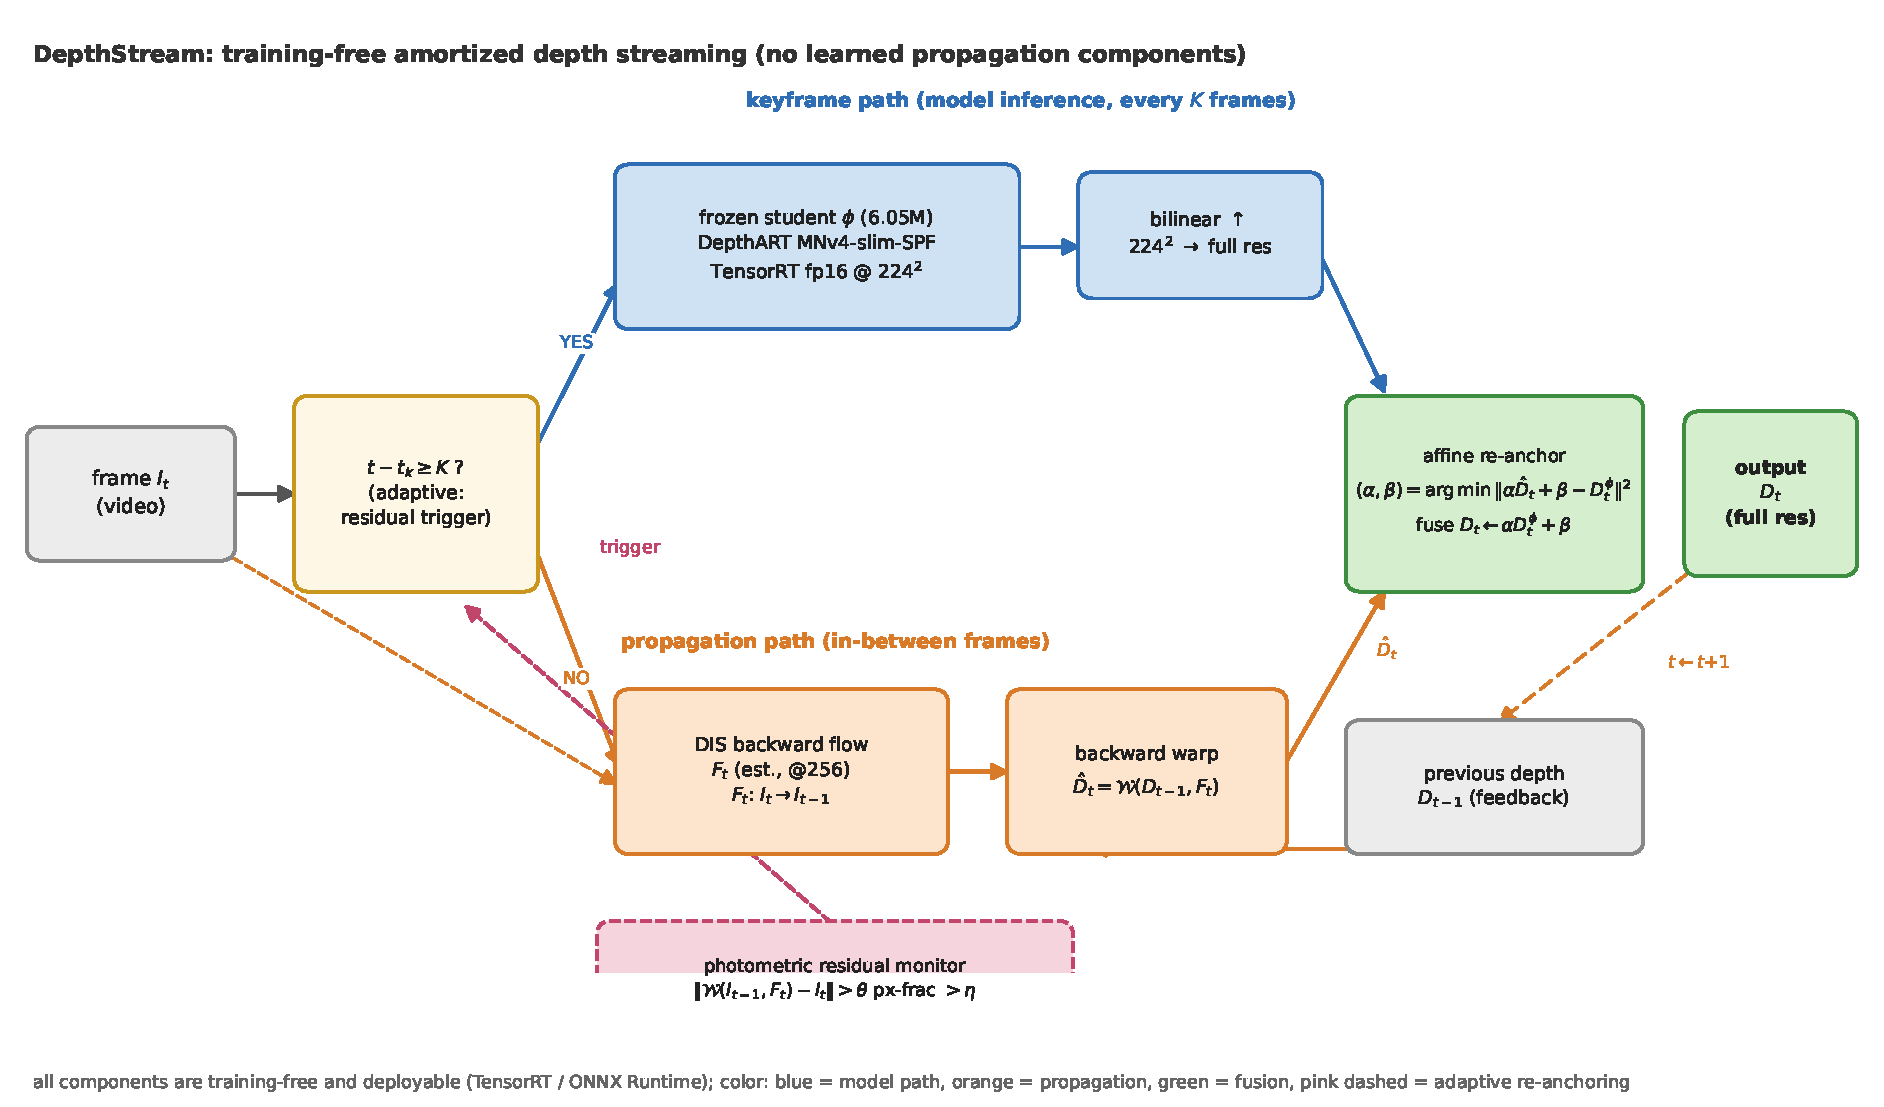
\includegraphics[width=\linewidth]{framework.pdf}
\caption{\textbf{DepthStream 运行时。}关键帧调度器把每帧路由到冻结学生（蓝）或经后向光流传播锚定深度场（橙）；仿射重锚定（绿）把时间连续性转移给新预测；光度残差监视器（粉、虚线）在光流失效处触发提前重锚定。没有任何组件被训练。}
\label{fig:framework}
\end{figure}

\begin{figure}[t]
\centering
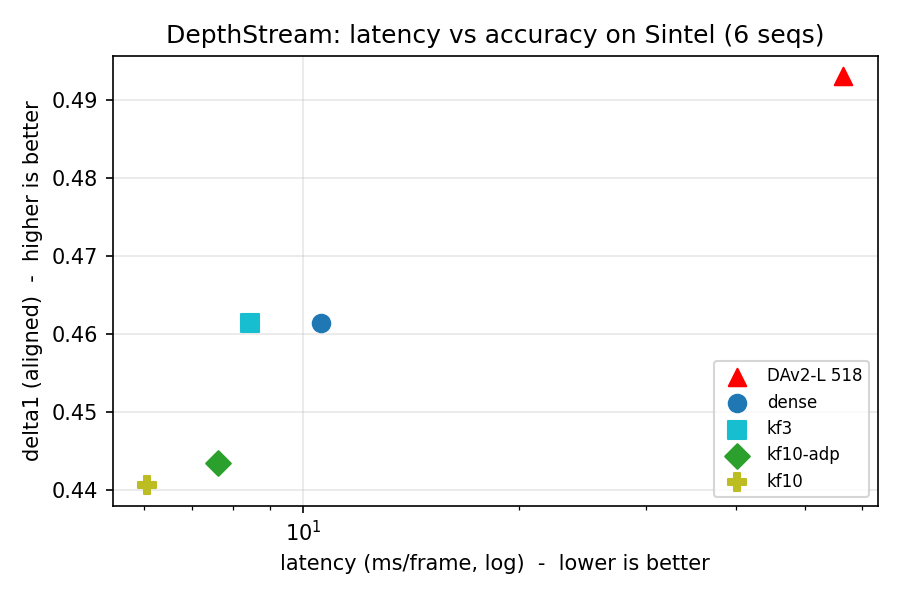
\includegraphics[width=0.85\linewidth]{pareto.png}
\caption{\textbf{延迟--精度平面}（Sintel）。DepthStream kf3 支配自身的逐帧基线；两者都以极小延迟坐在 $6.7\times$ 慢的教师的精度带上。紫色星标：Jetson Nano 节奏扫掠（640$^2$ 合成片段，仅延迟，纵向钉在同配置的 Sintel 精度上）——虚线在 kf3 与 kf10 之间穿过实时线。}
\label{fig:pareto}
\end{figure}

\begin{figure}[t]
\centering
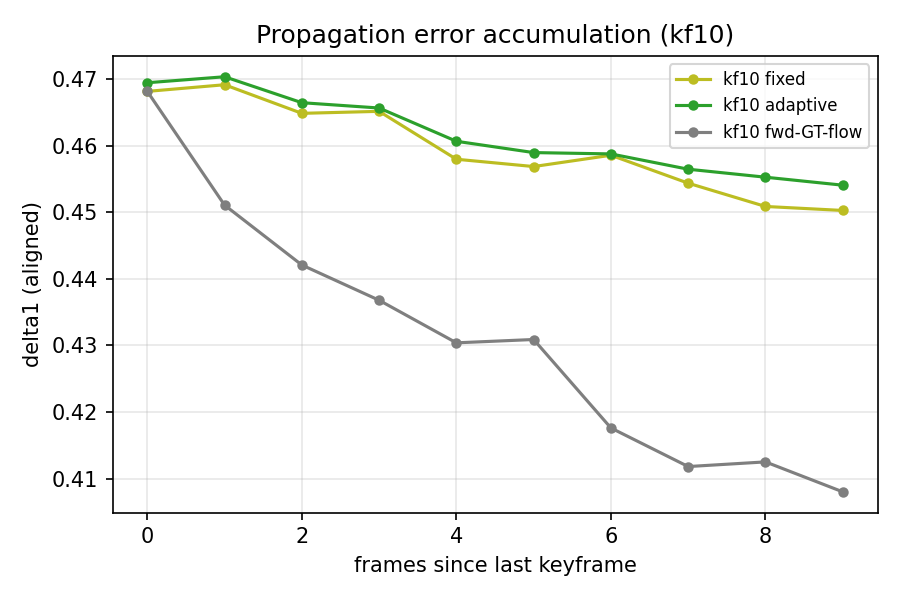
\includegraphics[width=\linewidth]{accum.png}
\caption{\textbf{传播衰减。}$\delta_1$ 对距上一关键帧帧数（Sintel）。自适应调度把衰减压平到九帧内 $-3.3\%$。}
\label{fig:accum}
\end{figure}

\subsection{时间稳定性：以 $\tau_5$ 复检}
\label{sec:tau5}
表~\ref{tab:perseqfull}列出全部配置的逐序列精度；逐序列方差（ambush\_2 的 0.03 到 market\_6 的 0.72）由场景内容主导，流式配置在 23 个序列中的 21 个上与逐帧对应值相差 $\pm 0.02$ 以内。

\begin{table}[t]
\centering\footnotesize
\setlength{\tabcolsep}{3pt}
\caption{\textbf{Per-sequence $\delta_1$} on all 23 Sintel sequences
(GT-capped protocol, TRT fp16 backend).}
\label{tab:perseqfull}
\begin{tabular}{lcccc}
\toprule
Sequence & dense & kf3 & kf10 & kf10-adp\\
\midrule
alley\_1 & 0.5992 & 0.5985 & 0.5673 & 0.5673 \\
alley\_2 & 0.1741 & 0.1775 & 0.1796 & 0.1796 \\
ambush\_2 & 0.0263 & 0.0294 & 0.0327 & 0.0327 \\
ambush\_4 & 0.3564 & 0.3602 & 0.3033 & 0.3666 \\
ambush\_5 & 0.0760 & 0.0737 & 0.0766 & 0.0766 \\
ambush\_6 & 0.4611 & 0.4352 & 0.3449 & 0.3449 \\
ambush\_7 & 0.9920 & 0.9912 & 0.9908 & 0.9908 \\
bamboo\_1 & 0.5883 & 0.5877 & 0.5762 & 0.5762 \\
bamboo\_2 & 0.2989 & 0.3046 & 0.2989 & 0.2989 \\
bandage\_1 & 0.6911 & 0.6971 & 0.6823 & 0.6823 \\
bandage\_2 & 0.5193 & 0.5273 & 0.5196 & 0.5196 \\
cave\_2 & 0.1406 & 0.1408 & 0.1450 & 0.1450 \\
cave\_4 & 0.2565 & 0.2630 & 0.2310 & 0.2310 \\
market\_2 & 0.2462 & 0.2481 & 0.2350 & 0.2350 \\
market\_5 & 0.3585 & 0.3592 & 0.3264 & 0.3264 \\
market\_6 & 0.1140 & 0.1115 & 0.1128 & 0.1128 \\
mountain\_1 & 0.6276 & 0.6276 & 0.5998 & 0.5998 \\
shaman\_2 & 0.6095 & 0.6093 & 0.5897 & 0.5897 \\
shaman\_3 & 0.9737 & 0.9739 & 0.9700 & 0.9700 \\
sleeping\_1 & 0.9363 & 0.9376 & 0.9370 & 0.9370 \\
sleeping\_2 & 0.7923 & 0.8011 & 0.7706 & 0.7706 \\
temple\_2 & 0.1721 & 0.1701 & 0.1490 & 0.1490 \\
temple\_3 & 0.6030 & 0.5875 & 0.4958 & 0.4958 \\
\bottomrule
\end{tabular}
\end{table}

\begin{table}[t]
\centering\footnotesize
\caption{\textbf{Per-sequence $\delta_1$} on the 9 Bonn RGB-D sequences
(Kinect GT, TRT fp32 backend). crowd saturates the metric because its
consecutive Kinect frames are near-duplicates.}
\label{tab:bonnperseq}
\begin{tabular}{lccc}
\toprule
Sequence & dense & kf3 & kf10-adp\\
\midrule
balloon & 0.9999 & 1.0000 & 1.0000 \\
balloon2 & 0.9368 & 0.9378 & 0.9105 \\
balloon\_tracking & 0.9954 & 0.9958 & 0.9958 \\
balloon\_tracking2 & 0.9916 & 0.9918 & 0.9926 \\
crowd & 1.0000 & 1.0000 & 1.0000 \\
crowd2 & 0.9686 & 0.9623 & 0.9434 \\
crowd3 & 0.9999 & 0.9999 & 0.9999 \\
kidnapping\_box & 0.9964 & 0.9967 & 0.9960 \\
kidnapping\_box2 & 0.9911 & 0.9910 & 0.9914 \\
\bottomrule
\end{tabular}
\end{table}


传播文献还报告 $\tau_5$~\cite{velodepth}：一种逐像素\emph{可靠率}——$t{-}1$ 的深度经光流扭曲到 $t$（GT 光流）、逐对尺度--平移对齐后，$|D_t - \widehat{D}_{t-1}|$ 小于深度 5\% 的像素记为一致。我们在无 ego-motion 项下实现 $\tau_5$（我们的运行时不消耗位姿；尺度--平移对齐吸收了主导修正），并在表~\ref{tab:tau5}报告全部 Sintel 配置。排序与 TAE 完全一致，但效应量更直观：流式把时间一致像素的份额从 55\%（dense）提升到 73\%（kf3）与 83\%（kf10-adp）——$1.5\times$ 的改进在换用对立指标族后依然成立。同协议下逐帧 DAv2-L 为 0.5516。

\begin{table}[t]
\centering\small
\caption{\textbf{$\tau_5$ 时间一致性}。上：Sintel（23 序列；GT 光流扭曲）。下：Bonn（9 序列；估计后向光流，各配置一致）。逐对尺度--平移对齐、5\% 可靠阈值；越高越好。}
\label{tab:tau5}
\begin{tabular}{lccc}
\toprule
配置 & dense & kf3 & kf10-adp\\
\midrule
Sintel（$\tau_5{\uparrow}$） & 0.5516 & 0.7332 & \textbf{0.8303}\\
Bonn（$\tau_5{\uparrow}$） & 0.8737 & 0.8786 & \textbf{0.8854}\\
\bottomrule
\end{tabular}
\end{table}

\subsection{午餐在哪里结束：节奏边界}
\label{sec:ksweep}
图~\ref{fig:ksweep}在全部 23 个 Sintel 序列上扫掠节奏 $K \in \{1,\dots,20\}$。延迟陡降后渐近（$12.4 \to 5.1$\,ms，$2.4\times$，下界为式~\ref{eq:cost}的光流项），时间误差单调下降——更长的传播链\emph{更平滑}——而精度温和且非单调地退化（$K{=}1$ 的 0.4614 到 $K{=}20$ 的 0.4297，$K{=}15$ 处的回弹可追溯到序列级方差而非共振效应）。一致性--延迟权衡的拐点在 $K{\approx}10$，我们将其作为自适应调度的默认值；$K{=}3$ 是保精度的替代。

\begin{figure}[t]
\centering
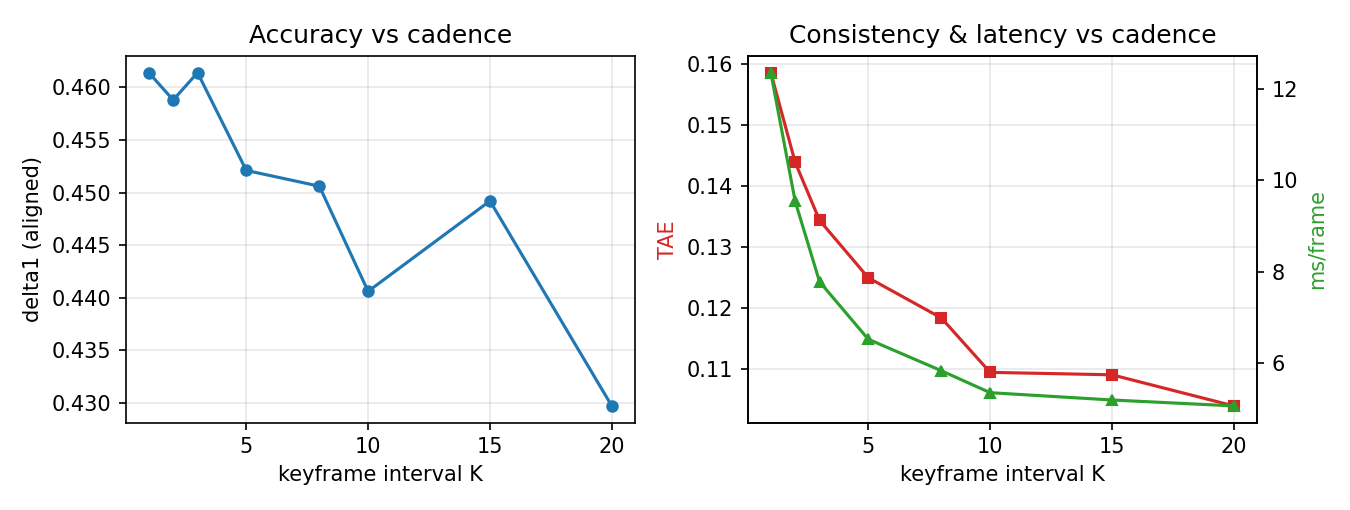
\includegraphics[width=\linewidth]{ksweep.png}
\caption{\textbf{节奏扫掠}（Sintel，23 序列，TRT fp16）。左：精度随 $K$ 温和非单调退化。右：时间误差（TAE，GT 光流）单调下降而延迟渐近于光流成本——拐点在 $K{\approx}10$。}
\label{fig:ksweep}
\end{figure}

\subsection{午餐为何免费：机制}
\label{sec:ablations}
表~\ref{tab:ablation}在 Sintel 上隔离每个设计决策；四条结论成立。

\begin{table}[t]
\centering\small
\setlength{\tabcolsep}{3.2pt}
\caption{\textbf{设计空间分析}（Sintel，23 序列）。"fwd-GT"以真值前向光流替换估计后向光流；"hi-flow"加倍光流处理宽度。}
\label{tab:ablation}
\begin{tabular}{lccc}
\toprule
变体 & $\delta_1{\uparrow}$ & TAE$\downarrow$ & ms$\downarrow$\\
\midrule
dense（逐帧） & 0.4614 & 0.1585 & 10.6\\
kf3（默认） & 0.4614 & 0.1343 & 8.4\\
kf3 + EMA（$\lambda{=}0.6$） & 0.4614 & 0.1345 & 8.6\\
kf10（固定） & 0.4406 & 0.1094 & 6.1\\
kf10-adp（自适应） & 0.4434 & 0.1054 & 7.6\\
kf10 + fwd-GT 光流 & 0.4145 & 0.1282 & 6.3\\
kf3 + hi-flow（384） & 0.4619 & 0.1354 & 9.4\\
\bottomrule
\multicolumn{4}{l}{\footnotesize EMA 的伤害是场景依赖的：在}\\
\multicolumn{4}{l}{\footnotesize 密林 ambush 子集上 $K{=}3$ 时 $\delta_1$}\\
\multicolumn{4}{l}{\footnotesize 从 0.2875 降至 0.2772。}\\
\end{tabular}
\end{table}

\textbf{(i) 时间 EMA 滤波有害——且是场景依赖的。}以指数滑动平均（$\lambda{=}0.6$）替换纯重锚定，会在每个关键帧把 $40\%$ 陈旧内容重新注入。在全部 23 序列协议下总体伤害温和（kf10-adp：0.4429 vs.\ 0.4434），但在含密林 ambush 序列的六序列子集上下降显著（$K{=}3$ 时 0.2875 降至 0.2772）：凡遮挡频繁处，陈旧的被传播内容就是错的，混合会把误差抹开。重锚定（式~\ref{eq:reanchor}）仅靠尺度--平移对齐获得连续性，在构造上稳健，故全文采用。

\textbf{(ii) 光流质量不是瓶颈。}用真值\emph{前向}光流传播的得分\emph{低于}估计的后向 DIS 光流（0.4145 vs.\ 0.4406）：前向光的坐标平移采样近似在遮挡处有偏，而后向光流恰定义在输出像素上。加倍光流分辨率同样中性（0.4619 vs.\ 0.4614）。传播误差由遮挡结构主导，而非光流精度——见图~\ref{fig:qual}的误差图，残差集中于运动边界。

\textbf{(iii) 自适应调度买回长间隔精度。}$K{=}10$ 下，自适应重锚定较固定调度恢复 $+0.021$ $\delta_1$（0.4434 vs.\ 0.4406），并取得全部配置最优时间误差（0.1054），代价 $+1$\,ms。值得注意的是，光度监视器在我们的基准上是\emph{休眠的安全网}：$\theta{=}0.15,\eta{=}0.30$ 下，Sintel 1{,}064 帧仅触发 1 次、Bonn 540 帧零次——DIS 光流几乎解释了全部观测运动——但单次重定时的关键帧会重排其整段序列的节奏，平均回收 $+0.003$ $\delta_1$。在生产流（含镜头切换、运动模糊、曝光变化）中，监视器的保险价值应显著更高，而我们的实验室基准对其表征不足。

\textbf{(iv) 几何（单应）传播是个陷阱。}RANSAC 单应分解——以主导静态运动扭曲、仅对残差用光流——在唯一旋转主导的序列上改善（temple\_2，相对 $+13\%$），但总体落败（四序列试点上 0.2776 vs.\ 0.2827 平均 $\delta_1$）：Sintel 的运动由前向平移主导，单一单应无法表达，而稠密后向光流隐式覆盖平移与旋转。无学习的稠密光流恰因不做运动模型假设而是强传播器。

\begin{figure}[t]
\centering
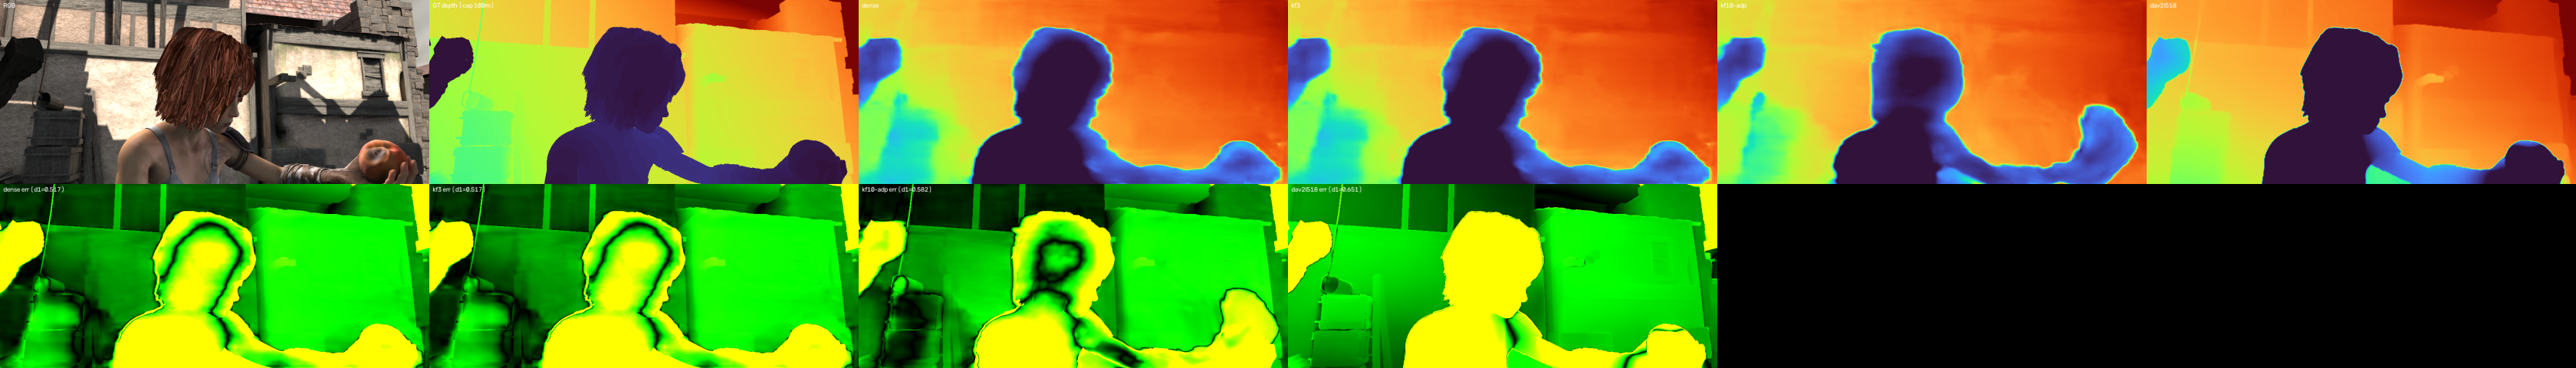
\includegraphics[width=\linewidth]{comparison_strip.png}\\[2pt]
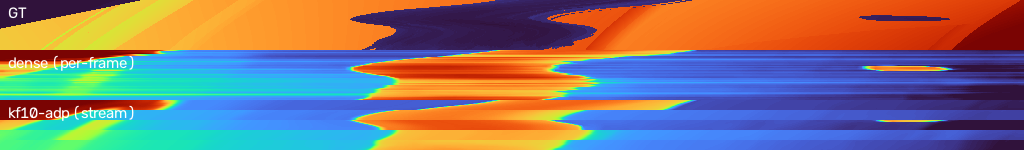
\includegraphics[width=\linewidth]{spacetime_slice.png}
\caption{\textbf{定性对比}（Sintel alley\_1）。上：RGB、真值与 dense、kf3、kf10-adp、教师的仿射对齐预测及误差图（$\delta_1$ 内嵌；绿=准确，红=相对误差 $>25\%$）。下：\textbf{时空切片}——一条扫描线的深度沿 50 帧堆叠。逐帧推理（中）闪烁；流式（下）形成平滑条带。}
\label{fig:qual}
\end{figure}

\begin{figure}[t]
\centering
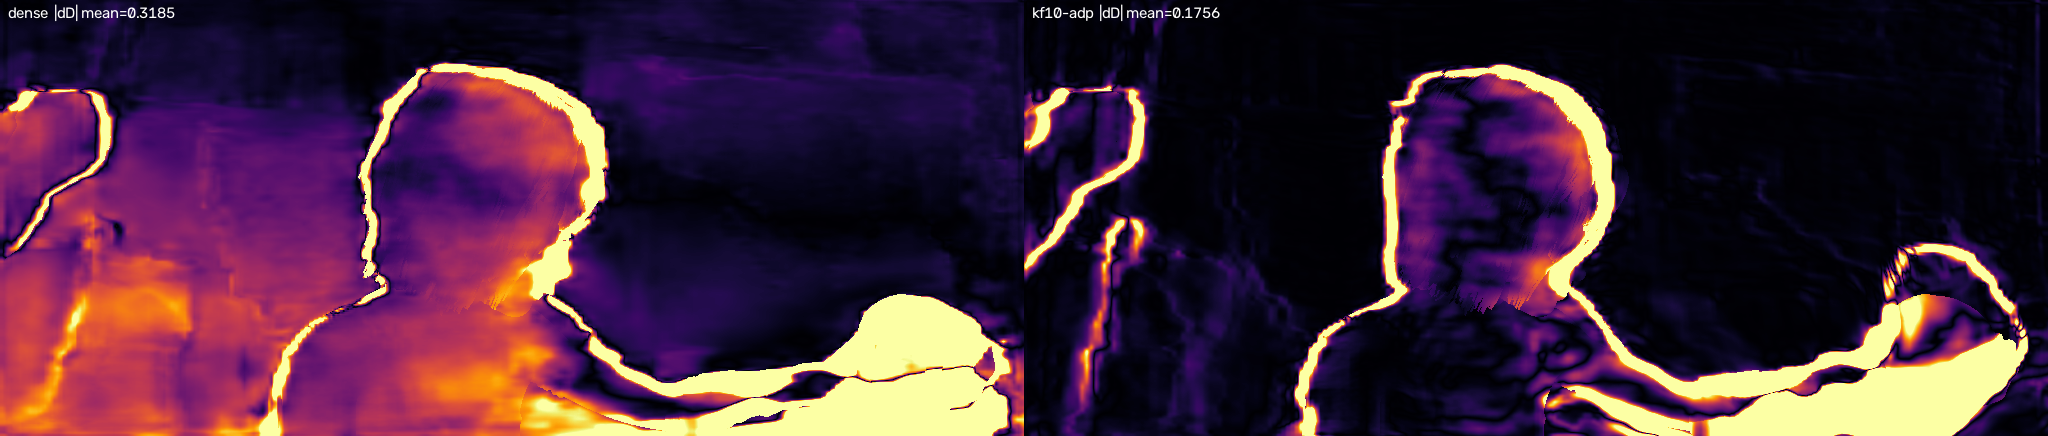
\includegraphics[width=\linewidth]{flicker_maps.png}
\caption{\textbf{帧间闪烁} $|D_t - \mathcal{W}(D_{t-1}, F^{gt})|$（Sintel，GT 光流扭曲）。流式将平均闪烁降低 45\%（0.3185 $\to$ 0.1756）；残差集中于运动边界——光流传播的预期失效模式。}
\label{fig:flicker}
\end{figure}

\begin{figure}[t]
\centering
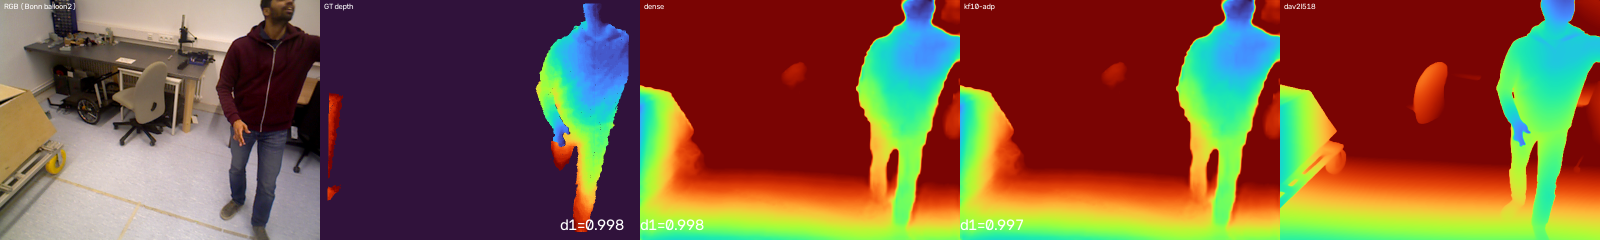
\includegraphics[width=\linewidth]{bonn_qual.png}
\caption{\textbf{真实数据}（Bonn balloon2）：RGB、Kinect 真值与仿射对齐预测。$\delta_1$ 内嵌：0.998 / 0.998 / 0.997。}
\label{fig:bonn}
\end{figure}

\begin{figure}[t]
\centering
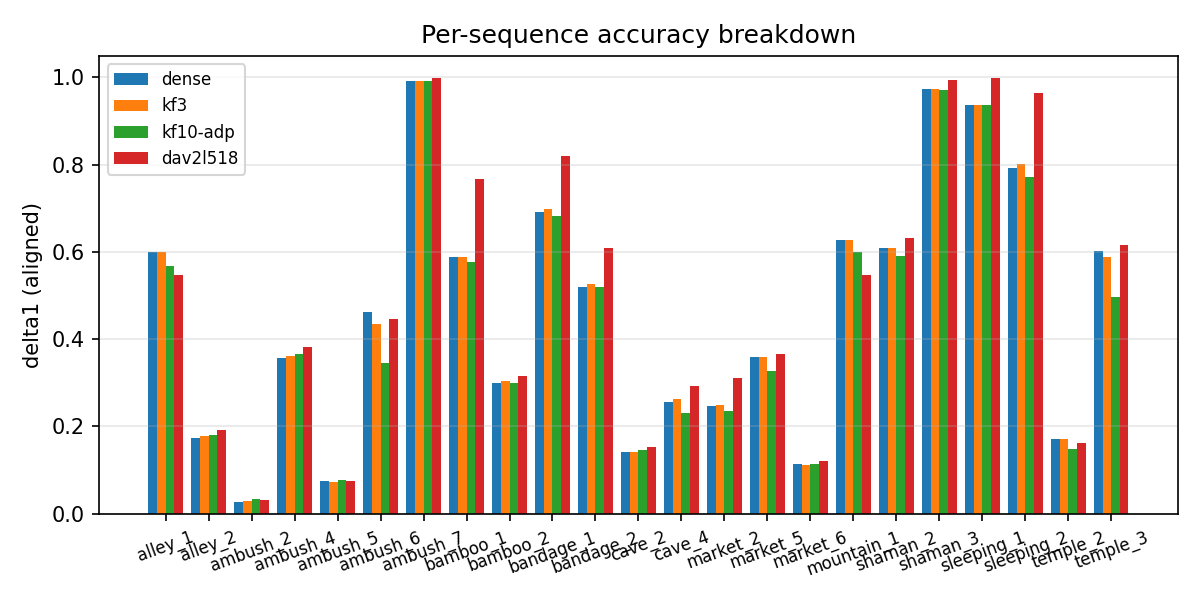
\includegraphics[width=0.8\linewidth]{perseq.png}
\caption{\textbf{逐序列精度}（Sintel，六序列协议）。序列级方差由场景难度主导（ambush 序列的密林），而非流式机制。}
\label{fig:perseq}
\end{figure}

\subsection{购买力：平台与后端不变性}
\label{sec:platform}
表~\ref{tab:platform}把评测延伸到多设备——从 2019 年 99 美元开发板到笔记本 GPU。CPU 运行 fp32 ONNX 图（4 线程）。部署上有三条主张：
(i)~\emph{精度后端不变}——全部配置下 fp32-CPU 与 fp16-GPU 的预测一致到 $\delta_1 \leq 10^{-4}$；
(ii)~\emph{摊销翻转 CPU 算术}——学生成本摊到十帧后，CPU 流不仅实时（$640{\times}480$ 端到端 249\,FPS），而且\emph{快于} GPU 流——因为推理被摊销后，逐帧瓶颈让位于光流与扭曲；
(iii)~\emph{2019 年的硬件也能实时}——在 Jetson Nano 4GB（Maxwell GPU，4\,GB 共享内存）上，逐帧推理只有 21\,FPS（$640{\times}480$），低于实时线，而 DepthStream kf10 达 90\,FPS（$4.2\times$）——同一运行时，其最近的学习式传播竞品~\cite{velodepth}的目标硬件是 RTX~3090。流场的跨设备一致率（Nano TRT fp32 vs.\ 桌面 ORT fp32，30 帧）为 Pearson $r{=}0.956$；残差反映平台专属引擎内核与光流数值差异，均被表~\ref{tab:main}与表~\ref{tab:ablation}的仿射不变协议吸收。

\begin{table}[t]
\centering\small
\caption{\textbf{平台}（学生后端；E2E 为 $640{\times}480$ 合成片段 kf10，Jetson 为 MAXN 功耗模式）。后端不变性：Sintel 协议上 GPU-fp16 与 CPU-fp32 的 $|\Delta\delta_1| \leq 10^{-4}$。Nano 节奏扫掠（逐帧/kf3/kf10/kf10-adp）：47.2/20.9/11.2/11.2\,ms = 21.2/47.9/89.6/89.6\,FPS（见图~\ref{fig:pareto}）。}
\label{tab:platform}
\begin{tabular}{llccc}
\toprule
平台 & 后端 & 精度 & 模型 & E2E kf10\\
\midrule
RTX 3060 Laptop 6GB & TensorRT 11.3 & fp16 & 1.20\,ms & $\sim$150 FPS\\
Ryzen 7 5800H（CPU） & ORT 1.26 & fp32 & 6.95\,ms & 249 FPS\\
Jetson Nano 4GB（2019） & TensorRT 8.2 & fp32 & 29.9\,ms & 90 FPS\\
\bottomrule
\end{tabular}
\end{table}

\begin{table}[t]
\centering\small
\caption{\textbf{分组件预算}（ms；$640{\times}480$）。model = 运行时实际执行的一次学生调用（预处理 + 主机--设备传输 + 引擎）；flow = 一次 256\,px DIS 场含上采样；warp = 全分辨率 remap。$224^2$ 下 Python 侧预处理在所有平台主导模型调用。}
\label{tab:components}
\begin{tabular}{lccc}
\toprule
平台 & model & flow & warp\\
\midrule
RTX 3060 Laptop（TRT fp16） & 12.4 & 2.2 & 0.8\\
Ryzen 7 5800H（ORT fp32） & 12.1 & 2.2 & 0.7\\
Jetson Nano（TRT fp32） & 46.6 & 7.3 & 1.0\\
\bottomrule
\end{tabular}
\end{table}

\subsection{分析：选择性精化何时划算？}
\label{sec:cascade}
摊销的天然竞争者是\emph{选择}：只在预期小模型出错处运行大教师。我们构建了这一投机级联运行时（翻转一致性与边缘线索选出 $16{\times}16$ 块的前 $p\%$；教师只对选中裁剪块推理；裁剪块经环带仿射对齐与羽化融合）。在 Sintel 上，学生已与教师在 93.6\% 像素上一致（以教师为参照的 $\delta_1$），我们测试的每个级联预算（10/20/40\%）都\emph{低于}纯学生、而延迟高 $70\times$——在本硬件上，裁剪级 ViT-L 推理摊销不过一次全图前向。负结果是有信息量的：蒸馏学生不给教师留下仲裁的分歧空间，这恰是建立在\emph{非蒸馏}基础模型上的传播系统~\cite{velodepth}需要学习修正的原因。选择是基础模型学生的正确工具；摊销是蒸馏学生的正确工具。

\subsection{负结果：基于单应的几何传播}
我们另实现了几何变体：稀疏光流对应上的 RANSAC 单应，静态内点区域用单应扭曲、其余用光流。它在唯一的旋转主导序列上改善（temple\_2，相对 $+13\%$ $\delta_1$），但总体落败（四序列试点平均 0.2776 vs.\ 0.2827）：Sintel 的相机运动由带强视差的前向平移主导，单一全局单应无法表达，而稠密后向光流均匀覆盖平移与旋转。无学习的稠密光流恰因不做运动模型假设而是强传播器。

%--------------------------------------------------------------------------
\section{讨论}
\label{sec:discussion}

\subsection{DepthStream vs.\ 学习式传播}
表~\ref{tab:velodepth}总结与最近系统的对比。两者互补而非竞争：VeloDepth 证明学习修正能从\emph{非蒸馏}基础基座挤出额外一致性；DepthStream 证明对从裁判蒸馏而来的学生，同一骨架——关键帧、扭曲、重锚——无需训练即可获得其收益的大部分，且延迟低一个数量级、硬件小 $7\times$。由我们的分析（\ref{sec:cascade}节）浮现的实用决策规则是：\emph{如果你的微型模型蒸馏自你的质量参照，传播——不要修正；重锚定——不要平滑。}

\begin{table}[t]
\centering\small
\caption{\textbf{DepthStream vs.\ 学习式传播}（VeloDepth 数字来自其论文；均为 0.3--0.5\,MP 输入）。}
\label{tab:velodepth}
\begin{tabular}{lcc}
\toprule
 & VeloDepth & DepthStream（本文）\\
\midrule
传播模块 & 55\,M，需训练 & 无\\
训练成本 & 8$\times$4090，6 天 & ---\\
基座模型 & 409\,M（UniDepthV2） & 6\,M 蒸馏\\
关键帧触发 & 学习门控 & 残差（免费）\\
硬件 & RTX 3090 & RTX 3060 Laptop 6GB\\
吞吐 & 26.2 FPS & 142--176 FPS\\
\bottomrule
\end{tabular}
\end{table}

\subsection{摊销何时停止划算？}
实验浮现出三条边界。\emph{遮挡密度}：传播误差集中于 disocclusion（图~\ref{fig:flicker}）；自适应调度在场景级掩蔽症状（提前重锚定），但逐像素掩码加回退推理是自然的下一步。\emph{极端间隔}：超过 $K{\approx}15$ 后累积曲线（图~\ref{fig:accum}）跌破 dense 基线，因此节奏应保持在衰减比模型自身帧间方差更平缓的范围内——本文经验为 $K{\leq}10$。\emph{模型错配}：若运行时的学生\emph{不是}从裁判模型蒸馏而来，分歧空间重新打开，选择性修正（\ref{sec:cascade}节）或学习式传播~\cite{velodepth}重新变得理性。

%--------------------------------------------------------------------------
\section{局限}
\label{sec:limits}
(i) 光流传播在 disocclusion 与大旋转处失效；自适应调度掩蔽症状（提前重锚定）但不显式建模遮挡。(ii) 评测覆盖一个合成与九个真实序列；把 Bonn 扩展到全部发布序列并加入 TUM 将加强真实数据主张。(iii) 平台表的功耗尚未报告；GPU 侧评测使用一台消费级笔记本 GPU；Orin 级 Jetson 结果预期可直接迁移（同一 TensorRT 流水线，DepthART 官方脚本存在）。(iv) 此处学生不消耗相机内参；DepthART 的度量变体需要将 $K$ 与场一起传播。(v) VeloDepth~\cite{velodepth} 报告的时间一致性指标（$\tau^{\mathrm{SSI}}_5$）我们尚未复现其 ego-motion 项，因此与它的对比是架构与延迟层面的，而非指标精确的。

%--------------------------------------------------------------------------
\section{结论}
对一个蒸馏到最后一滴参数的深度模型，剩余效率在时间维度——而且可以免费收割。DepthStream 在关键帧上运行冻结的 6\,M 学生，用后向光流搬运锚定深度场，用闭式仿射拟合重锚定新预测；光度监视器守护调度。免费午餐真实且严格：$K{=}3$ 时流式在精度上与逐帧完全一致，同时降低延迟并把时间一致像素从 55\% 提升到 73\%——在合成与真实基准上皆然。午餐有绘制的边界——节奏拐点 $K^*{\approx}10$、混合的遮挡惩罚、一个蒸馏条件——其购买力翻转部署版图：2019 年 99 美元的板子上 90\,FPS 稳定深度、CPU 上 249\,FPS、两种后端精度相同。给从业者的规则只有一句话：传播——不要修正；重锚定——不要平滑。

%--------------------------------------------------------------------------
\section*{可复现性与许可}
全部表格由单命令产出（\texttt{eval\_sintel\_v2.py}、\texttt{eval\_bonn.py}、\texttt{bench\_cpu.py}；图由 \texttt{plots.py}、\texttt{qual\_figs.py}、\texttt{draw\_framework.py} 产出）。学生权重与教师权重公开；学生及其部分监督继承 DepthART 与 Depth Anything V2 的 CC BY-NC 4.0 条款，限制所发布权重的商业使用（运行时本身无此限制）。Sintel 与 Bonn 按各自研究许可使用。

% 参考文献保留英文（学术惯例），与英文版一致
\begin{thebibliography}{25}\small
\bibitem{depthart} F.~Xue et al. ``DepthART: Scaling Foundation Monocular Depth to Tiny Models,'' \emph{ACM Multimedia}, 2026. arXiv:2607.17099.
\bibitem{dav2} L.~Yang et al. ``Depth Anything V2,'' \emph{NeurIPS}, 2024. arXiv:2406.09414.
\bibitem{velodepth} L.~Piccinelli et al. ``Video Depth Propagation (VeloDepth),'' \emph{3DV}, 2026. arXiv:2512.10725.
\bibitem{nvds} W.~Wang et al. ``Neural Video Depth Stabilizer,'' \emph{ICCV}, 2023.
\bibitem{depthcrafter} W.~Cao et al. ``DepthCrafter: Generating Consistent Long Depth Sequences for Open-world Videos,'' \emph{CVPR}, 2025.
\bibitem{chronodepth} J.~Shao et al. ``Learning Temporally Consistent Video Depth from Video Diffusion Models'' (ChronoDepth), \emph{CVPR}, 2025.
\bibitem{vda} S.~Chen et al. ``Video Depth Anything: Consistent Depth Estimation for Super-Long Videos,'' \emph{CVPR}, 2025. arXiv:2501.12375.
\bibitem{cvd} J.~Kopf et al. ``Consistent Video Depth Estimation,'' \emph{ACM TOG (SIGGRAPH)}, 2021.
\bibitem{teccvideodepth} S.~Li, Y.~Luo, Y.~Mao et al. ``Enforcing Temporal Consistency in Video Depth Estimation'' (TCMonoDepth), \emph{ICCV Workshops}, 2021.
\bibitem{midas} R.~Ranftl et al. ``Towards Robust Monocular Depth Estimation: Mixing Datasets for Zero-shot Cross-dataset Transfer,'' \emph{IEEE TPAMI}, 2022.
\bibitem{da1} L.~Yang et al. ``Depth Anything: Unleashing the Power of Large-Scale Unlabeled Data,'' \emph{CVPR}, 2024. arXiv:2401.10891.
\bibitem{zoedepth} S.~F.~Bhat et al. ``ZoeDepth: Zero-shot Transfer by Combining Relative and Metric Depth,'' \emph{ICRA}, 2023.
\bibitem{marigold} B.~Ke et al. ``Repurposing Diffusion-based Image Generators for Monocular Depth Estimation,'' \emph{CVPR}, 2024.
\bibitem{depthfm} M.~Gui et al. ``DepthFM: Fast Monocular Depth Estimation with Flow Matching,'' \emph{ACM Multimedia}, 2024.
\bibitem{rtmonodepth} M.~Pietruszka et al. ``Real-Time Monocular Depth Estimation on Embedded Systems,'' \emph{arXiv:2308.10569}, 2023.
\bibitem{dff} X.~Zhu et al. ``Deep Feature Flow for Video Recognition,'' \emph{CVPR}, 2017.
\bibitem{xmem} C.~Cheng and M.~Schiele. ``XMem: Long-Term Video Object Segmentation with an Atkinson-Shiffrin Memory Model,'' \emph{ECCV}, 2022.
\bibitem{specdec} Y.~Leviathan et al. ``Fast Inference from Transformers via Speculative Decoding,'' \emph{ICML}, 2023.
\bibitem{practicalcvd} P.~Li, Y.~Ding, L.~Li, J.~Guan, and Z.~Li. ``Towards Practical Consistent Video Depth Estimation,'' \emph{ACM ICMR}, 2023.
\bibitem{metric3d} W.~Yin et al. ``Metric3D v2: Geometric Foundation Model,'' \emph{IEEE TPAMI}, 2024.
\bibitem{unidepth} L.~Piccinelli et al. ``UniDepth: Universal Monocular Metric Depth Estimation,'' \emph{CVPR}, 2024.
\bibitem{fastdepth} D.~Wofk et al. ``FastDepth: Efficient Monocular Depth Estimation for Embedded Devices,'' \emph{ICRA}, 2019.
\bibitem{patchfusion} Z.~Li et al. ``PatchFusion: An End-to-End Tile-Based Framework for High-Resolution Monocular Metric Depth Estimation,'' \emph{CVPR}, 2024.
\bibitem{disflow} T.~Kroeger et al. ``Fast Optical Flow using Dense Inverse Search,'' \emph{ECCV}, 2016.
\bibitem{farneback} G.~Farneb\"ack. ``Two-Frame Motion Estimation Based on Polynomial Expansion,'' \emph{SCIA}, 2003.
\bibitem{sintel} D.~J.~Butler et al. ``A Naturalistic Open Source Movie for Flow Evaluation,'' \emph{ECCV}, 2012.
\bibitem{bonn} E.~Palazzolo et al. ``ReFusion: 3D Reconstruction in Dynamic Environments using a Time-of-Flight Sensor'' (Bonn RGB-D Dynamic), \emph{IROS}, 2019.
\bibitem{dpt} R.~Ranftl et al. ``Vision Transformers for Dense Prediction'' (DPT), \emph{ICCV}, 2021.
\bibitem{mobilenetv4} D.~Qin et al. ``MobileNetV4 -- Universal Models for the Mobile Ecosystem,'' \emph{arXiv:2404.10518}, 2024.
\bibitem{tensorrt} NVIDIA. ``TensorRT,'' \url{https://developer.nvidia.com/tensorrt}.
\end{thebibliography}

\end{document}
